\documentclass{article}
% Change "article" to "report" to get rid of page number on title page
\usepackage{amsmath,amsfonts,amsthm,amssymb}
\usepackage{setspace}
\usepackage{Tabbing}
\usepackage{fancyhdr}
\usepackage{lastpage}
\usepackage{extramarks}
\usepackage{chngpage}
\usepackage{soul,color}
\usepackage{graphicx,float,wrapfig}
\usepackage{multirow}
\usepackage{enumerate}
% In case you need to adjust margins:
\topmargin=-0.45in      %
\evensidemargin=0in     %
\oddsidemargin=0in      %
\textwidth=6.5in        %
\textheight=9.0in       %
\headsep=0.25in         %

% Homework Specific Information
\newcommand{\hmwkTitle}{ME p.k. Gibbs Sampling}
\newcommand{\hmwkClass}{}
\newcommand{\hmwkAuthorName}{Donglai\ Wei}


% Setup the header and footer
\pagestyle{fancy}                                                       %
\lhead{\hmwkAuthorName}                                                 %
\rhead{\firstxmark}                                                     %
\lfoot{\lastxmark}                                                      %
\cfoot{}                                                                %
\rfoot{Page\ \thepage\ of\ \pageref{LastPage}}                          %
\renewcommand\headrulewidth{0.4pt}                                      %
\renewcommand\footrulewidth{0.4pt}                                      %

% This is used to trace down (pin point) problems
% in latexing a document:
%\tracingall

%%%%%%%%%%%%%%%%%%%%%%%%%%%%%%%%%%%%%%%%%%%%%%%%%%%%%%%%\begin{enumerate}

% Some tools
\newcommand{\enterProblemHeader}[1]{\nobreak\extramarks{#1}{#1 continued on next page\ldots}\nobreak%
                                    \nobreak\extramarks{#1 (continued)}{#1 continued on next page\ldots}\nobreak}%
\newcommand{\exitProblemHeader}[1]{\nobreak\extramarks{#1 (continued)}{#1 continued on next page\ldots}\nobreak%
                                   \nobreak\extramarks{#1}{}\nobreak}%

\newlength{\labelLength}
\newcommand{\labelAnswer}[2]
  {\settowidth{\labelLength}{#1}%
   \addtolength{\labelLength}{0.25in}%
   \changetext{}{-\labelLength}{}{}{}%
   \noindent\fbox{\begin{minipage}[c]{\columnwidth}#2\end{minipage}}%
   \marginpar{\fbox{#1}}%

   % We put the blank space above in order to make sure this
   % \marginpar gets correctly placed.
   \changetext{}{+\labelLength}{}{}{}}%

\setcounter{secnumdepth}{0}
\newcommand{\homeworkProblemName}{}%
\newcounter{homeworkProblemCounter}%
\newenvironment{homeworkProblem}[1][Problem \arabic{homeworkProblemCounter}]%
  {\stepcounter{homeworkProblemCounter}%
   \renewcommand{\homeworkProblemName}{#1}%
   \section{\homeworkProblemName}%
   \enterProblemHeader{\homeworkProblemName}}%
  {\exitProblemHeader{\homeworkProblemName}}%

\newcommand{\problemAnswer}[1]
  {\noindent\fbox{\begin{minipage}[c]{\columnwidth}#1\end{minipage}}}%

\newcommand{\problemLAnswer}[1]
  {\labelAnswer{\homeworkProblemName}{#1}}

\newcommand{\homeworkSectionName}{}%
\newlength{\homeworkSectionLabelLength}{}%
\newenvironment{homeworkSection}[1]%
  {% We put this space here to make sure we're not connected to the above.
   % Otherwise the changetext can do funny things to the other margin

   \renewcommand{\homeworkSectionName}{#1}%
   \settowidth{\homeworkSectionLabelLength}{\homeworkSectionName}%
   \addtolength{\homeworkSectionLabelLength}{0.25in}%
   \changetext{}{-\homeworkSectionLabelLength}{}{}{}%
   \subsection{\homeworkSectionName}%
   \enterProblemHeader{\homeworkProblemName\ [\homeworkSectionName]}}%
  {\enterProblemHeader{\homeworkProblemName}%

   % We put the blank space above in order to make sure this margin
   % change doesn't happen too soon (else \sectionAnswer's can
   % get ugly about their \marginpar placement.
   \changetext{}{+\homeworkSectionLabelLength}{}{}{}}%

\newcommand{\sectionAnswer}[1]
  {% We put this space here to make sure we're disconnected from the previous
   % passage

   \noindent\fbox{\begin{minipage}[c]{\columnwidth}#1\end{minipage}}%
   \enterProblemHeader{\homeworkProblemName}\exitProblemHeader{\homeworkProblemName}%
   \marginpar{\fbox{\homeworkSectionName}}%

   % We put the blank space above in order to make sure this
   % \marginpar gets correctly placed.
   }%

%%%%%%%%%%%%%%%%%%%%%%%%%%%%%%%%%%%%%%%%%%%%%%%%%%%%%%%%%%%%%



%%%%%%%%%%%%%%%%%%%%%%%%%%%%%%%%%%%%%%%%%%%%%%%%%%%%%%%%%%%%%
% Make title
\title{\vspace{0.3in}\textmd{\textbf{\hmwkTitle}}}
\date{2010.6.14}
\author{\textbf{\hmwkAuthorName}}
%%%%%%%%%%%%%%%%%%%%%%%%%%%%%%%%%%%%%%%%%%%%%%%%%%%%%%%%%%%%%

\begin{document}
\begin{spacing}{1.1}
\maketitle

\section{0)Outline}
\begin{enumerate}
\item ME: From Split to Decompose
\item Gibbs: when to fail
\end{enumerate}


\section{1) ME for Dirichlet-Multinomial}
\subsection{i) Formula}
W:number of unique words\\ 
$n_{..k}$number of customers in dish k \\
$n_{..k}^{w}$number of occurence of word w in dish k \\
$n_{j..}$number of customers in in Restaurant j \\
$n_{jt.}$number of customers in table t in Restaurant j \\
$m_{..}$number of tables in total \\
$m_{.k}$number of tables in dish k \\

$-P=-log p(x,z|\lambda)$\\ =\\
(t-term)$ \underline{log \frac{\Gamma(m_{..}+\gamma)}{\Gamma(\gamma)}+\sum_{j=1}^{J} \{log \frac{\Gamma(n_{j..}+\alpha)}{\Gamma(\alpha)}-\sum_{t=1}^{m_{j.}}[log(\Gamma(n_{jt.})+log \alpha
]\}}$\\ \\
+(k-term)$ \sum_{k=1}^{K} [log(\frac{\Gamma(n_{..k}+W\phi_{0})}{\Gamma(W\phi_{0})})+log(\Pi_{w=1}^{W}\frac{\Gamma(\phi_{0})}{\Gamma(\phi_{0}+n_{..k}^{w})})
-\underline{log(\Gamma(m_{.k})-log \gamma]}$\\ \\ 
=\\
(z-term)$ +\sum_{k=1}^{K} [log(\frac{\Gamma(n_{..k}+W\phi_{0})\Gamma(\phi_{0})^{W}}{\Gamma(W\phi_{0})\Pi_{1}^{W}\Gamma(\phi_{0}+n_{..k}^{w})\Pi_{t^{*}=1}^{m_{.k}}\Gamma(n_{.t^{*}k})})]$\\ \\
(m-term)$-m_{..}log\alpha+log\frac{\Gamma(m_{..}+\gamma)}{\Pi_{k=1}^{K}\Gamma(m_{.k})}$\\ \\
(constant-term)$-log\Gamma(\gamma)+\sum_{j=1}^{J} log \frac{\Gamma(n_{j..}+\alpha)}{\Gamma(\alpha)}$
\\ 
=\\
(table-res-term)$\sum_{j=1}^{J} log \frac{1}{\Pi_{t=1}^{m_{j.}}\alpha\Gamma(n_{jt.})}$\\ \\
(table-dis-term)$\sum_{k=1}^{K} log \frac{\Gamma(n_{..k}+W\phi_{0})\Gamma(\phi_{0})^{W}}{\Pi_{1}^{W}\Gamma(\phi_{0}+n_{..k}^{w})\gamma\Gamma(W\phi_{0})}$\\ \\
(table-num-term)$log \frac{\Gamma(m_{..}+\gamma)}{\Pi_{t=1}^{m_{j.}}\Gamma(m_{.k})}$\\ \\
(constant-term)$-log\Gamma(\gamma)+\sum_{j=1}^{J} log \frac{\Gamma(n_{j..}+\alpha)}{\Gamma(\alpha)}$
\\ \\
\subsection{ii) Comparison:Split v.s. Decompose}
\subsubsection{a)Intuition}
i)Intuitively, Split-Merge is designed for Gaussian case, where a cluster should be defined as group of points close to each other. \\
ii)It is natural to do split move in the Euclidean space, where it is kind of "transive".(e.g. if cluster 1 should be splitted into
three clusters, it may still be better off if we first split it into 2 clusters.
)\\ \\
But for Dirichlet-Multinomial case:\\
i) the Sample Space itself is discrete.\\
ii)The aim is to find a reasonable size of topics to {\bf explain} the raw documents.\\ \\
\subsubsection{b)Strategy}
The Goal of ME algorithm is to search for the best assignment variable $\vec z$ that maximize the log probability P.\\ \\
The basic idea is to search {\bf "locally"},changing the config of a table/restaurant/dish conditioned on others fixed.\\
\begin{enumerate}
\item Given other Restaurants fixed, want to find the best Restaurant j's Config:\\
1)Split:2-means++(sampling dishes) $m_{j.}\rightsquigarrow 2*m_{j.}$ +TKM \\
2)Decompose: samples the dish component+TKM
\item Given other dishes fixed, want to find the best Dish k's Config:\\
1)Split:2-means++(sampling dishes) $m_{.k}\rightsquigarrow m_{.k}+1$ +TKM \\
2)Decompose: samples the dish component+TKM
\end{enumerate}
Obviously, the Decompose move is much more flexible.
\subsubsection{c)Problem with Split}
1) Senario 1:(Noisy Dishes) If several dishes(mixture of 2 bars) share some bars, it will be hard to figure out the true bar by split dishes {\bf sequentially}.\\
2) Senario 2:(Multiple Bars) If one dish is made of multiple bars, the {\bf two} new splitted dishes won't be explained well by other bars. \\
Solution:(which is kind of nasty even for toy data)\\
1)Split-Dish-All\\
2)Split-Dish-Further\\
\subsection{iii) Decompose move}
\subsubsection{a)Decompose Restaurant}
\begin{enumerate}[(i)]
\item Decompose Restaurant j:
\begin{enumerate}
\item Iterate until no customers are left 
\item For each dish k:calculate the weight of forming a table(with dish k) with the overlapped words in the restaurant  
\item Sample the table according the weight and make it 
\end{enumerate}
\item TKM
\end{enumerate}
{\bf NOTE:}:\\
During Initialization: TKM enables new table/dish;weight is $\Delta$P\\
During Search:TKM doesn't allow new table/dish;weight is $\Delta\frac{\Gamma(m_{..}+\gamma)}{\Pi_{1}^{W}\Gamma(\phi_{0}+n_{..k}^{w})}$\\\\

\subsubsection{b)Decompose Dish}
\begin{enumerate}[(i)]
\item Decompose each table(into 1 or 2 tables) in dish k:
\begin{enumerate}
\item Remove the table t from the restaurant
\item For each dish K$\neq$k:calculate the weight of forming a table(with dish k) with the overlapped words in the table   
\item Sample the table according the weight and make it 
\item make the rest of the words in the table back to table t.
\item Local Search table
\end{enumerate}
\item Split-k
\item TKM
\end{enumerate}
{\bf NOTE:}:\\
Decompose Table:weight is $\Delta\frac{\Gamma(m_{..}+\gamma)}{\Pi_{1}^{W}\Gamma(\phi_{0}+n_{..k}^{w})}$\\
During Initialization: TKM enables new table/dish\\
During Search:TKM doesn't allow new table/dish\\

\subsection{iv) Experiment on 200 Restaurants(5*5)}
Algorithm:\\
while until P doesn't increase:\\
1)Decompose Restaurant(Initialization)\\
2)Decompose Dish(Initialization)\\
while until P doesn't increase:\\
3)Decompose Restaurant(Search)\\
4)Decompose Dish(Search)\\
End\\
End\\
\begin{figure}[h] 
  \begin{minipage}[b]{0.5\textwidth} 
    \centering 
    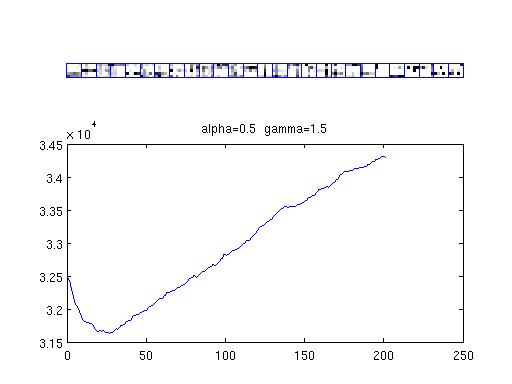
\includegraphics[width=2.5in,height=2in]{200_initr.jpg} 
    \caption{1)DR Initialization}
    \label{fig:by:table} 
  \end{minipage}% 
  \begin{minipage}[b]{0.5\textwidth} 
    \centering 
    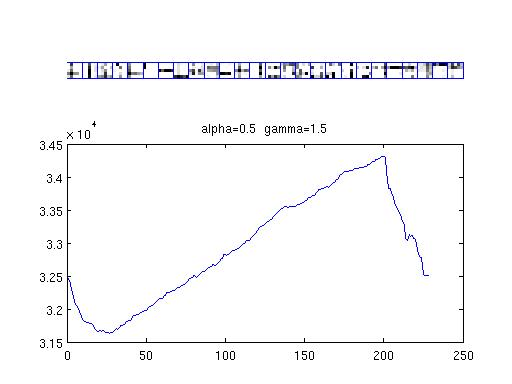
\includegraphics[width=2.5in,height=2in]{200_initrd.jpg} 
    \caption{2)DD Initialization}
    \label{fig:by:table}  
   \end{minipage}% 
\end{figure}
\begin{figure}[h] 
  \begin{minipage}[b]{0.5\textwidth} 
    \centering 
    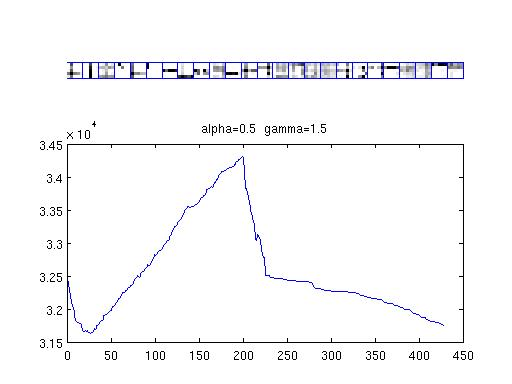
\includegraphics[width=2.5in,height=2in]{200_initrd_r1.jpg} 
    \caption{3)DR Search}
    \label{fig:by:table} 
  \end{minipage}% 
  \begin{minipage}[b]{0.5\textwidth} 
    \centering 
    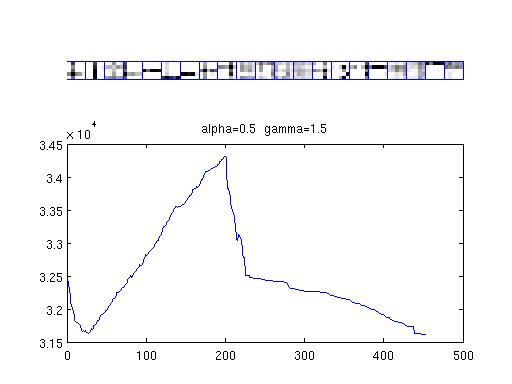
\includegraphics[width=2.5in,height=2in]{200_initrd_r1_d1.jpg} 
    \caption{4)DD Search}
    \label{fig:by:table}  
   \end{minipage}% 
\end{figure}
\begin{figure}[h] 
  \begin{minipage}[b]{0.5\textwidth} 
    \centering 
    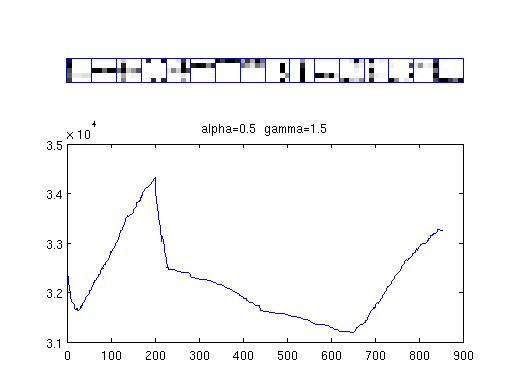
\includegraphics[width=2.5in,height=2in]{200_initrd_r1_d1_r1_rr.jpg} 
    \caption{1)DR Initialization}
    \label{fig:by:table} 
  \end{minipage}% 
  \begin{minipage}[b]{0.5\textwidth} 
    \centering 
    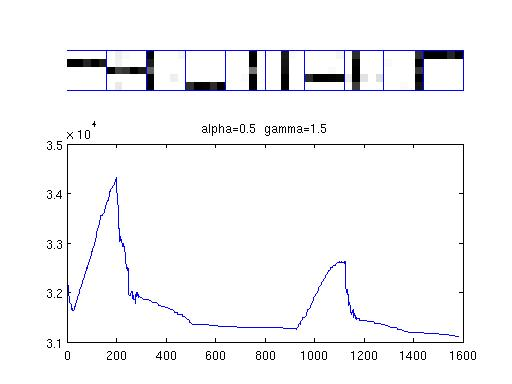
\includegraphics[width=2.5in,height=2in]{200_initrd_r1_d1_r1_rr_ddd.jpg} 
    \caption{Finally...}
    \label{fig:by:table}  
   \end{minipage}% 
\end{figure}

\section{2) Gibbs}
Problems for Gibbs:\\
\begin{enumerate}
\item Hard to decide when to stop
\item Quick to find the bars, but hard to purify them with large moves

\subsection{i)Comparison on 200 Restaurants(5*5)}
From Teh's package 1.0, test Gibbs sampling methods: crf,beta,block.\\

\begin{figure}[h] 
  \begin{minipage}[b]{0.5\textwidth} 
    \centering 
    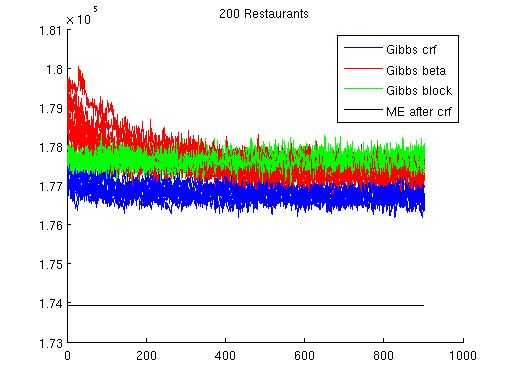
\includegraphics[width=2.5in,height=2in]{200compare.jpg} 
    \caption{comparison}
    \label{fig:by:table} 
  \end{minipage}% 
  \begin{minipage}[b]{0.5\textwidth} 
    \centering 
    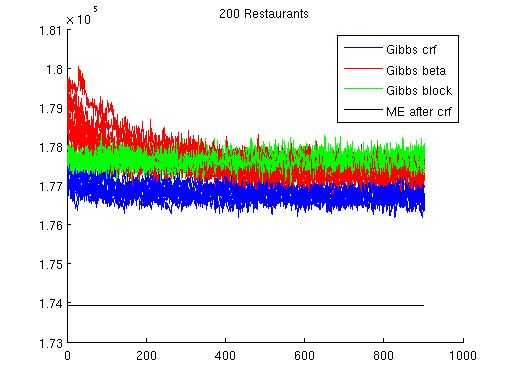
\includegraphics[width=2.5in,height=2in]{200compare.jpg} 
    \caption{Finally...}
    \label{fig:by:table}  
   \end{minipage}% 
\end{figure}



\end{enumerate}


\end{spacing}
\end{document}

%%%%%%%%%%%%%%%%%%%%%%%%%%%%%%%%%%%%%%%%%%%%%%%%%%%%%%%%%%%%%
